\documentclass{article} % For LaTeX2e
\usepackage{nips13submit_e,times}
\usepackage{hyperref}
\usepackage{url}
%\documentstyle[nips13submit_09,times,art10]{article} % For LaTeX 2.09
\usepackage{graphicx}
\graphicspath{ {/Users/abhimanyu/GitHub/Project_cs224D/mnist(Projectcode&poster)/report/report/} }
\usepackage{amssymb}

\title{Knowledge extraction from medical literature using Recurrent Neural Networks}


\author{
Abhimanyu Banerjee\thanks{ Use footnote for providing further information
about author (webpage, alternative address)---\emph{not} for acknowledging
funding agencies.} \\
Department of Physics\\
Stanford  University\\
Stanford, CA  \\
\texttt{manyu@stanford.edu} \\
/
/
}

% The \author macro works with any number of authors. There are two commands
% used to separate the names and addresses of multiple authors: \And and \AND.
%
% Using \And between authors leaves it to \LaTeX{} to determine where to break
% the lines. Using \AND forces a linebreak at that point. So, if \LaTeX{}
% puts 3 of 4 authors names on the first line, and the last on the second
% line, try using \AND instead of \And before the third author name.

\newcommand{\fix}{\marginpar{FIX}}
\newcommand{\new}{\marginpar{NEW}}

%\nipsfinalcopy % Uncomment for camera-ready version

\begin{document}


\maketitle

\begin{abstract}
The problem of extracting knowledge relationships from unstructured text has proved a challenge for NLP. 
We focus on extracting relationship information between drugs targeting bacteria from medical literature. Deep learning 
techniques have proved most fruitful of late in learning relationships from NLP tasks.
We use a recurrent neural network architecture (LSTM) and use this to train on labeled sentences to decide whether a given relationship exists

\end{abstract}

\section{Introduction}
Extracting knowledge and summarizing knowledge from reading unstructured text remains one of the large challenges in NLP. In this 
project I have focused on extracting medical relationships from bio-medical literature. A complete repository of relationships such as gene-gene, gene-drug, bacteria-drug will be extremely helpful for better understanding drug response$[3]$. The number of known and curated gene-gene relations is growing exponentially and is cataloged in databases such as BioGRID and ChEA. Medical literature itself is growing every year at a rapid rate and curating it by humans is too slow, so it would be really useful if we had a tool that could automatically curate these relationships for us. To be a little more concrete, I have focused on extracting relationships between drugs targeting bacteria . If we are given a sentence with a drug and a bacteria, we want to be able to say whether the drug has any action in targeting the bacteria. Deciding this is a 
challenge as context matters a lot. Below are two examples to illustrate this point.


\begin{figure}[h]
\begin{center}
%\framebox[4.0in]{$\;$}
%\fbox{\rule[-.5cm]{0cm}{4cm} \rule[-.5cm]{4cm}{0cm}}
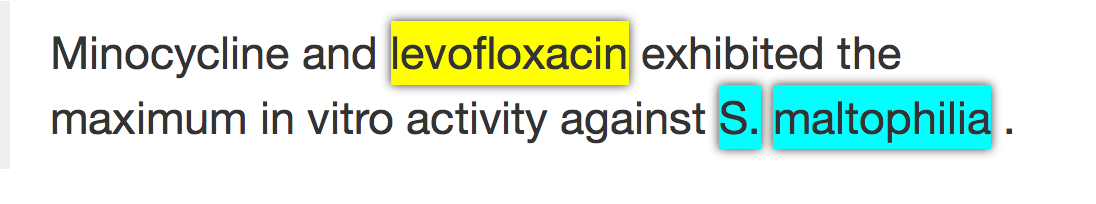
\includegraphics[width = 0.7\linewidth]{postive_example.png}
\end{center}
\caption{Drug(Levifloxacin) targets bacteria(S.maltophilia) is a a positive example}
\end{figure}

\begin{figure}[h]
\begin{center}
%\framebox[4.0in]{$\;$}
%\fbox{\rule[-.5cm]{0cm}{4cm} \rule[-.5cm]{4cm}{0cm}}
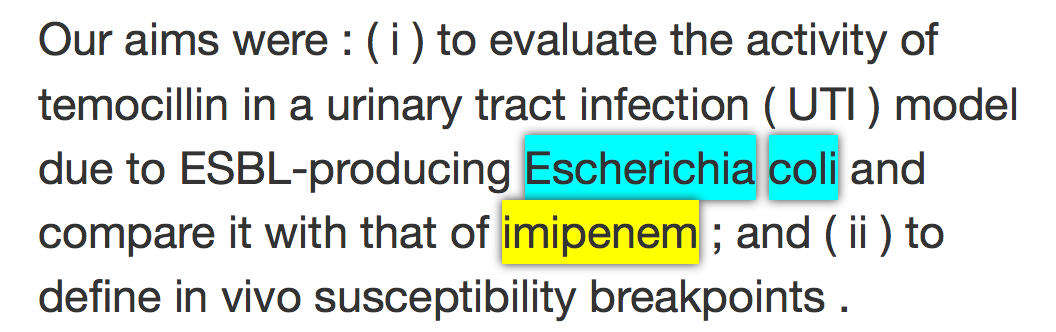
\includegraphics[width = 0.7\linewidth]{negative_example.png}
\end{center}
\caption{Ipipenem and Escherichia Coli. It is not clear what their relationship is . A negative example}
\end{figure}

The first example is a clear sentence from which we can read and say that Levifloxacin definitely targets the bacteria S.maltophilia . The second example is vague and there is no clear evidence of Ipipenem acting on Escherichia Coli. We want to learn examples such as the first and pick out such relationships(ie. Levifloxacin acts on S.maltophilia) and ignore examples such as the second as it does not reveal anything insightful. \\
Deep learning approaches have been applied to several NLP tasks such as language modeling[4], sequence to sequence learning[5] with great successes. The natural architecture for learning on sequences is a reccurent neural network (RNN) or some variant of it. We use an LSTM architecture to learn on our data .

\section{Dataset and pre-processing data}
Since there is not dataset of labeled sentences with drugs targeting bacteria, I had to create my own dataset for this purpose. I used the tool called [6]\textbf{ddlite} developed by Chris Re's group which is useful in rapid prototyping and extracting relations. Ddlite was very useful in setting up the dataset. I first downloaded a corpus of $14388$ articles containing bacteria and drug mention keywords from Pubmed central.
After downloading this, I extracted all sentences that contain both a drug name and a bacteria name from a dictionary match . I got a total of $7001$ such sentences. We call such a sentence as a "relation mention" . The "relation-mentions" now need to be labeled with a positive or a negative label depending on whether they exhibit a target sort of relationship between the drug and the bacteria or not.\\
To do this, we must write rules which we call "Labeling functions " in ddlite. Each Labeling function is a rule that assigns the sentence a $+1$ label if the relation exhibited meets the condition of a positive target relation, labels $-1$ if the sentence meets the condition of a negative relation and $0$ if the labeling function is not conclusive and can not decide. These rules have to be designed well to pick out good examples as we do not want to add noisy labels which will affect our final training. We also want large "coverage" ie. our rules should be able to give a $+1$ or a $-1$  label to a large fraction of our data set. We do not want too many $0$ labels as these are useless for training. \\

I have written several rules($59$ of them) that do labeling and got  a coverage of about $60\%$ , ie. I am able to label $60\%$ of these sentences with a positive or a negative label.  Some examples of labeling functions are: If we find the words "target","degrade","infect","conducive" in the sentence between the drug and bacteria , mark these sentences with a $+1$. Some examples of negative labeling functions: If the bacteria and drug are too far apart in the sentence, separated by $ >20$ tokens, mark it with a $-1$ as it is unlikely they have any relation. Often also things like chemical elements and nucleotides are mentioned as drugs, mark these as negative examples as well. \\
Finally it may happen that a sentence may have several different labels, because of different labeling functions clashing. In this case we take  a majority vote and assign a single label to the sentence. After doing this I finally generated a computer labeled dataset of  $2157$ sentences. Of this $906$ have the label $+1$ and $1251$ have the label $-1$ . \\
We hope that this dataset is good enough for training a deep learning model that would capture language features and from that learn what a postive or a negative example would look like. I split this dataset to $1600$ for training, $300$ for testing hyper-parameters and $257$ for my development set.

\subsection{pre training word-vectors}
I created a vocabulary of word embedding trained specifically for this task on Medical literature. I used a subset of the Medline corpus containing several thousand medical abstracts. The size of this corpus in all was $1.5GB$ and I got it from the lab I work in (Russ Altman's lab). The word vectors were trained using Tensorflows version of word2vec with skipgram and throwing out ultra rare tokens which occur $<5$ times in the corpus. The dimension of the word embeddings is $128$. \\
Since the word embeddings generated contain both bacteria and drugs, I first did an initial experiment to see if there is any clustering of concepts ie. do well formed concepts such as a bacteria and a drug emerge from these word embeddings and can we visualize them? I plotted the $2D$ PCA of the top $100$ most frequently occuring drugs and bacteria for this purpose.\\

\begin{figure}[h]
\begin{center}
%\framebox[4.0in]{$\;$}
%\fbox{\rule[-.5cm]{0cm}{4cm} \rule[-.5cm]{4cm}{0cm}}
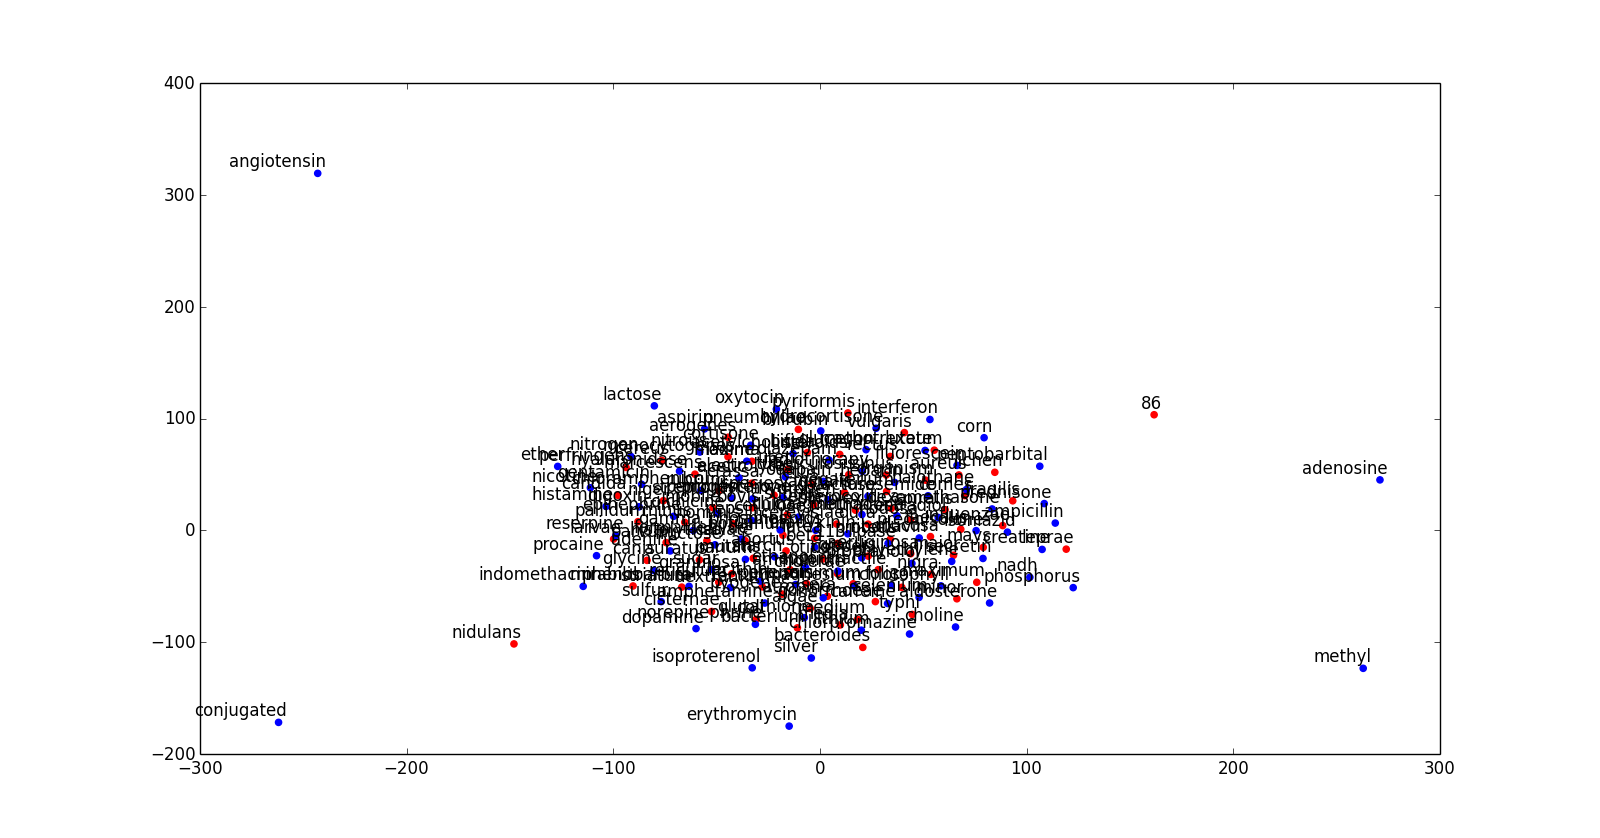
\includegraphics[width = 0.7\linewidth]{w2v.png}
\end{center}
\caption{$2D $ PCA of top $100$ most frequent bacteria and drugs. Bacteria are in red and drugs are in blue}
\end{figure}


The word embedding do not cluster well on meaning. As you can see from the figure, the clusters overlap a lot . The data-set for training word vectors is probably not large enough to have formed these well developed concepts.


\section{Approach}
We use the recurrent neural network architecture framework because this is what is quite natural when you have sequential data. RNNs are very successful in learning on large sequences and modeling the sequences. We use a popular version of the RNN called as the LSTM (long short term memory) 
\subsection{Model-\textbf{LSTM} recurrent neural networks:}
The LSTM (long short term memory ) are a modified kind of recurrent neural networks. They were introduced by Hochreiter and Schmidhuber $(1997)$[7] , and have been successfully used by many people in following work . They work tremendously well on a large variety of problems, and are now widely used. 
Vanilla RNN's can learn long term dependencies in principle but do not work well in practice. This is because they suffer from the problem of vanishing and exploding gradients. The LSTM solves this problem elegantly by defining a cell state that is a linear combination of a new state and the previous state. This allows it to remember information across several time steps and in practice has much better performance. The wonderful review article by Christopher Olah explains the concepts behind LSTM quite well [2].
The basic structure of the LSTM is shown in the picture below in figure $4$:

\begin{figure}[h]
\begin{center}
%\framebox[4.0in]{$\;$}
%\fbox{\rule[-.5cm]{0cm}{4cm} \rule[-.5cm]{4cm}{0cm}}
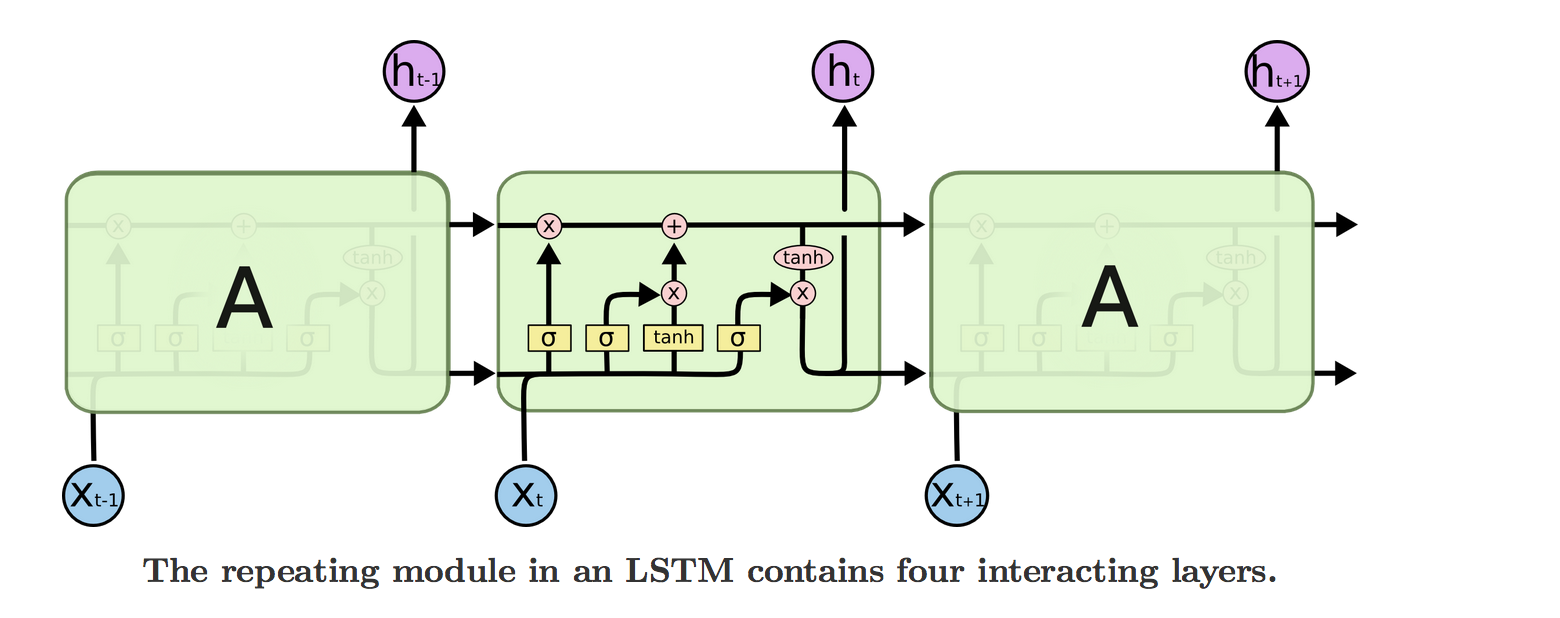
\includegraphics[width = 0.8\linewidth]{LSTM.png}
\end{center}
\caption{An unrolled LSTM recurrent neural network}
\end{figure}

The state of the LSTM is referred to by the symbol $C_t$ This is updated at every step according to the update rules. The final hidden state
$h_t$ is got from the cell state.

\subsection{The LSTM update equations:}
The LSTM has 3 gates , a forget gate , an input gate and an output gate. The forget gate controls how much of the previous state we want to keep, the input gate regulates how important the current input information is and the output gate regulates the output. It is best understood by the equations:
\begin{equation}
f_t=\sigma(W_f.[h_{t-1},x_{t}]+b_f)
\end{equation}
Here $f_t$ is the forget gate, $W_f \in \mathbb{R}^{(n*n)}$  and $b_f \in \mathbb{R}^{(n)}$.\\
Similarly we also have an input gate and an update state:
\begin{eqnarray}
i_t=\sigma(W_i.[h_{t-1},x_{t}]+b_i)\\
\tilde{C_t}=Tanh(W_c[h_{t-1},x_{t}]+b_c)
\end{eqnarray}
Here as before $W_i \in \mathbb{R}^{(n*n)}$,$W_c \in \mathbb{R}^{(n*n)}$,$b_i \in \mathbb{R}^{(n)}$,$b_c \in \mathbb{R}^{(n)}$
The input and forget gates act to determine how much of the old state to forget and how much of the new state to use to develop the output state . \\

\begin{equation}
C_t=f_t \circ C_{t-1}+ i_t \circ \tilde{C_t}
\end{equation}
\begin{eqnarray}
o_t=\sigma(W_o.[h_{t-1},x_{t}]+b_o) \\
h_t=o_t \circ Tanh(C_t)
\end{eqnarray}

Finally the output gate acts on the final state to produce the current hidden state. The output gate controls what it decides is important to outputted to the hidden state. Of course $W_o \in \mathbb{R}^{(n*n)}$ and $b_o \in \mathbb{R}^{(n)}$ \\
It is the final hidden state that we are interested in. The complicated dynamics of creating this state allows the LSTM to solve the vanishing, exploding gradient problems and learn well over long time steps.\\
We finally feed the final hidden state to a softmax layer (with two output states) and train the neural network with the Cross Entropy cost for the Softmax layer. 






\section{Experiment:}
We train the LSTM using the cross entropy cost of the final hidden state. I modified a version of the LSTM code available to train MNIST [8]. Since tensorflow requires you to enter the number of steps in an RNN from before, you need to pad the sentences to a fixed length. What this means is that a special 'PAD' symbol must be introduced in the embedding which is a zero vector. All shorter sentences than the padded length must have the 'PAD' symbol at the end to make it of the fixed length. Larger sentences will get cut off. The average length of a sentence in my dataset was $38$ tokens.
The padded length is a hyper parameter that must be varied to get optimum performance.
\subsection{Values of the hyper parameters used and tuned}
Each word in the dictionary has a fixed length of $128$ . \\
The dimension of the hidden state is $200$ .Performance did not change with changing it to $256$ \\
Total epochs : $15$ or $20$\\
Number of steps is varied between $10$ to $150$. The average sentence length is  $38$ \\
Learning rate : $.001$\\
Batch size : $30$\\

I used the Adam optimizer to optimize.

\section{Results:}
Since my training set is small ($1800$) sentences, the model overfits on the training data. The model is quite sensitive to the length of the padded sentence used (the number of steps) . I got the best performance for number of steps equal to $50$ with a classification accuracy of $65 \%$ on the \textbf {dev. set}.
I have plotted the performance of the classification algorithm on the dev. set as a function of the number of steps used in figure$5$.
\begin{figure}[h]
\begin{center}
%\framebox[4.0in]{$\;$}
%\fbox{\rule[-.5cm]{0cm}{4cm} \rule[-.5cm]{4cm}{0cm}}
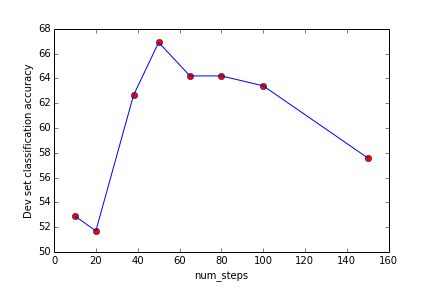
\includegraphics[width = 0.8\linewidth]{classification_accuracy.png}
\end{center}
\caption{Classification accuracy on the dev set as a function of the number of steps used}
\end{figure}

It is interesting that we have a peak performance near the average sentence length of my data. Very small lengths are expected to be bad 
as we cut off too much information. Very long sentence lengths get confused on the shorter sentences as they have too many trailing zeros from the padding. Due to this they get stuck in local minima that they can't come out of and do not have good performance. I have also plotted the dev set accuracy as a function of number of training epochs. This turned out to be quite instructive and we can see how the sentences which are padded to larger lengths get stuck in local minima of the cost during training and the accuracy does not change much(unless it jumps abruptly out of the minima)\\

\begin{figure}[h]
\begin{center}
%\framebox[4.0in]{$\;$}
%\fbox{\rule[-.5cm]{0cm}{4cm} \rule[-.5cm]{4cm}{0cm}}
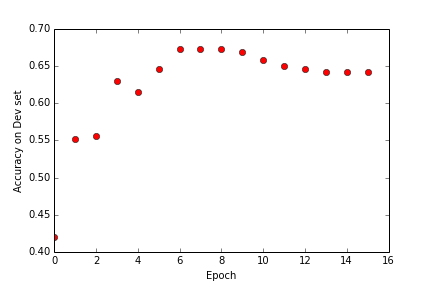
\includegraphics[width = 0.8\linewidth]{dev_accuracy_65.png}
\end{center}
\caption{Classification accuracy on the dev set as a function training epoch and sentence length= $65$}
\end{figure}

\begin{figure}[h]
\begin{center}
%\framebox[4.0in]{$\;$}
%\fbox{\rule[-.5cm]{0cm}{4cm} \rule[-.5cm]{4cm}{0cm}}
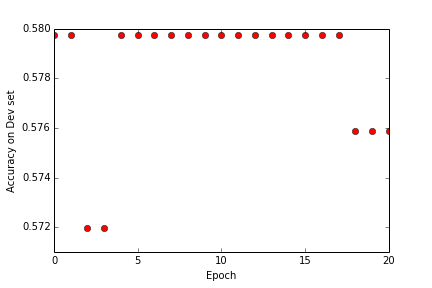
\includegraphics[width = 0.8\linewidth]{dev_accuracy_150.png}
\end{center}
\caption{Classification accuracy on the dev set as a function training epoch and sentence length= $150$. Note how the accuracy randomly jumps from one local minima to another}
\end{figure}


The shorter padded sentence length of $65$ shows increasing accuracy (on dev set) with training epochs. The large padded length of $150$ shows no improvement from one epoch to the next. It is stuck in local minimas. However it jumps out of one local minima only to be stuck in another.

\section{Conclusions}
Our LSTM model is clearly able to learn as we have about $65\%$ classification on the dev.set . However we are limited by our data which is computer generated so, we do not know whether it is learning actual relationships or just fitting the rules I have defined with my labeling functions. It will be amazing to have a good human labeled dataset for this purpose. 



\subsubsection*{Acknowledgments}

I really wish to thank my friend Raunaq for helping out with the project and homework. This course would not have been as much fun without his help. I also want to thank Emily Mallory for helping me learn ddlite and being a mentor.  Thanks to Yuhao Zhang for giving me the medline data to train word vectors and being there to discuss different deep learning models.

\subsubsection*{References}


\small{
[1] Wojciech Zaremba \& Ilya Sutskever \& Oriol Vinyals (2014) Recurrent Neural Network Regularization
 {\it arXiv:1409.2329}

[2] Christopher Olah -Understanding LSTM Networks {\it{http://colah.github.io/posts/2015-08-Understanding-LSTMs}/ }

[3] Emily Mallory \& Ce Zhang \& Chris Re \& Russ Altman(2015) Large-scale extraction of gene interactions from full-text literature using DeepDive {\it Bioinformatics first published online September 3, 2015 doi:10.1093/bioinformatics/btv476 }

[4]Tomas Mikolov \& Martin Karafiat \& Lukas Burget \& Jan "Honza" Cernocky \& Sanjeev Khudanpur - Recurrent neural network based language model {\it INTERSPEECH. Vol. 2. 2010}

[5]Sutskever Ilya \& Oriol Vinyals and Quoc V. Le. "Sequence to sequence learning with neural networks."{\it Advances in neural information processing systems. 2014.}

[6]DDLITE by Chris Re et. al {\it https://github.com/HazyResearch/ddlite}

[7]Hochreiter, Sepp, \& Jürgen Schmidhuber. "Long short-term memory."{\it  Neural computation 9.8 (1997): 1735-1780.}

[8]https://github.com/aymericdamien/TensorFlow-Examples

\end{document}
